\documentclass[11pt]{article}

\usepackage[margin=1in]{geometry}
\usepackage[T1]{fontenc}
\usepackage{lmodern}
\usepackage{amsmath}
\usepackage{xcolor}
\usepackage{listings}
\usepackage{booktabs}
\usepackage{longtable}
\usepackage{enumitem}
\usepackage{upquote}
\usepackage{microtype}
\usepackage{hyperref}
\hypersetup{colorlinks=true, linkcolor=blue!50!black, urlcolor=blue!50!black}
\usepackage{tikz}
\usetikzlibrary{arrows.meta,positioning,shapes,fit,calc}

\lstdefinestyle{code}{
  language=C,
  basicstyle=\ttfamily\small,
  columns=fullflexible,
  keepspaces=true,
  breaklines=true,
  frame=single,
  numbers=none,
  showstringspaces=false,
}
\lstdefinelanguage{Curry}{
  morekeywords={case,of,let,in,where,data,free,if,then,else,fcase,external,import,module},
  sensitive=true,
  morecomment=[l]{--},
}
\lstset{style=code}

% Keep -- as two hyphens in code, and let lines stretch around long
% identifiers, which can't be hyphenated.
\DisableLigatures[-]{encoding = T1, family = tt*}
\setlength{\emergencystretch}{3em}

% \code and \file print their argument verbatim, so underscores are fine.
% Don't put # or % in them.
\newcommand{\code}[1]{\texttt{\detokenize{#1}}}
\newcommand{\file}[1]{\nolinkurl{#1}}

\title{The Rice Developer's Manual}
\author{Steven Libby}
\date{}

\begin{document}
\maketitle

\begin{abstract}
Rice is an optimizing compiler from Curry to C.  This manual is for anyone who
wants to work on it.  It explains how the source tree is organized, what each
pass of the compiler does and why, what the generated C looks like, and how the
runtime system evaluates it: the graph of nodes, the evaluation machine, the
trail we backtrack with, and the garbage collector.  Read it before the code.
The comments in the code explain individual functions and point back here for
the bigger ideas.
\end{abstract}

\tableofcontents

%======================================================================
\section{Introduction}
%======================================================================

\subsection{What Rice is}

Curry is a functional logic language.  It looks a lot like Haskell, with two
additions that drive almost every design decision in Rice:
\begin{itemize}
  \item \textbf{Nondeterminism.}  \code{x ? y} can be either \code{x} or
    \code{y}.  A program can have several results, and we find them by trying
    one alternative, and backtracking to try the other.
  \item \textbf{Free variables.}  A variable can be unknown, and get bound
    later, either by unification (\code{x =:= Just 3}) or by
    \emph{narrowing}: when a case expression looks at a free variable, we guess
    each constructor in turn.
\end{itemize}
Like Haskell, Curry is lazy, so we only evaluate what we need.

Rice doesn't parse Curry itself.  The standard Curry front end (the one KiCS2 and
PAKCS use) turns a Curry module into \emph{typed FlatCurry}, a small, explicitly
typed core language.  Rice reads that, optimizes it, turns it into ICurry (an
imperative intermediate language from the \code{icurry} package), and writes C,
which is compiled together with Rice's runtime system into an ordinary
executable.

Rice itself is written in Curry, and is built and run with KiCS2.

If Curry is new to you, the Curry language report and the tutorials at
\url{https://curry-lang.org} are the place to start.  For FlatCurry and ICurry,
see the documentation of the \code{flatcurry}, \code{flatcurry-typed} and
\code{icurry} packages (\url{https://cpm.curry-lang.org}), and the paper
``ICurry'' by Antoy, Hanus, Jost and Libby (WFLP 2019).

\subsection{Where things are documented}

We write three kinds of documentation, and each has its own home
(\file{STYLE_GUIDE.md}, ``Three kinds of comments''):
\begin{enumerate}
  \item \textbf{What the code does} is in comments in the code.
  \item \textbf{How the pieces fit together, and why} is in this manual.
  \item \textbf{History}: bugs we fixed, things we tried and dropped,
    measurements.  That's in \file{src/compiler-history.md},
    \file{src/runtime-history.md} and the plan documents in \file{src/}
    (\S\ref{sec:docs}).
\end{enumerate}
\file{STATUS.md} and \file{current.md} record what state the project is in.

%======================================================================
\section{Getting started}
%======================================================================

\subsection{Building Rice}

You need KiCS2 (Rice is a KiCS2 program), the Curry package manager
\code{cypm}, Haskell Stack (or cabal) for the front end, and clang (or gcc,
with \code{--gcc}).  From the project root,
\begin{lstlisting}[language=bash]
git submodule update --init
make CYPM=~/opt/kics2/bin/cypm
\end{lstlisting}
builds the front end into \file{bin/} (\code{make frontend}, about 12 minutes
the first time), installs \code{rice} into \file{~/.cpm/bin}
(\code{make rice}), and compiles Prelude (\code{make prelude}).  While working
on the compiler, rebuild just \code{rice} with
\begin{lstlisting}[language=bash]
PATH=~/opt/kics2/bin:$PATH cypm install
\end{lstlisting}
Put KiCS2 first on your \code{PATH}: \code{cypm} builds with whichever Curry
system it finds, and Rice is only tested built with KiCS2.

At run time Rice finds its standard library (\file{lib/}), its runtime
(\file{runtime/}) and its Prelude replacements (\file{replace/}) in the
directory it was installed from.  Set \code{RICEHOME} to use another copy.
Rice also needs a Curry front end (\S\ref{sec:frontend}).

\subsection{Running it}

\begin{lstlisting}[language=bash]
rice Prog.curry                # builds ./Prog; main :: IO t runs once
rice --interactive Prog.curry  # main can have any type; prints every solution
\end{lstlisting}
\code{rice --help} lists the options.  The ones you'll use most while working
on the compiler print an intermediate stage: \code{-f} (FlatCurry),
\code{-u} (after unboxing), \code{-r} (after replacing), \code{-o} (after the
optimizer), \code{--printANF}, \code{-i} (ICurry), and
\code{--print-fieldreps}.  \code{--stop-...} prints a stage and stops.
\code{--trace-optimize} prints every rewrite the optimizer makes.
\code{--compiler-time} times each stage.

Options for the generated program:
\begin{itemize}
  \item \code{--debug=low|med|high} builds with tracing (\file{runtime/debug.h}).
    It also turns on the field rep lint (\S\ref{sec:fieldreps}).
  \item \code{--cflags="..."} passes flags to the C compiler, usually to change
    a runtime flag: \code{--cflags=-DOPT_EPOCH_TRAIL=1}.
  \item \code{--force-recompile} and \code{--force-recompile-module=M} ignore
    the caches (\S\ref{sec:caching}).
\end{itemize}

\subsection{Running the tests}

\begin{lstlisting}[language=bash]
tests/run.sh              # the regression tests; run before every commit
tests/run.sh regressions  # only tests whose path contains "regressions"
tests/run.sh --slow       # also the large benchmarks
tests/optbench.sh         # what each backtracking optimization buys
\end{lstlisting}
\file{tests/README.md} describes the test bench in detail
(\S\ref{sec:testing}).

\subsection{Runtime flags worth knowing}

These are C preprocessor flags, set with \code{--cflags}:
\begin{center}
\begin{tabular}{@{}ll@{}}
\toprule
\code{-DOPT_...=0/1} & turn a backtracking optimization on or off (\S\ref{sec:opts}) \\
\code{-DOPT_STATS=1} & count trail entries, retries, forward hops, \dots; print at exit \\
\code{-DGC_STRESS} & collect at every safe point, and poison freed memory \\
\code{-DGC_STATS} & print a line for each collection \\
\code{-DCHECK_LAYOUT=1} & check every node built by \code{make_X}/\code{set_X} \\
\bottomrule
\end{tabular}
\end{center}

%======================================================================
\section{The source tree}
%======================================================================

\subsection{Directories}

\begin{longtable}{@{}p{0.28\textwidth}p{0.68\textwidth}@{}}
\toprule
\file{src/Rice/} & the compiler (\S\ref{sec:compiler}) \\
\file{src/FlatCurry/} & typed versions of FlatCurry libraries we need but
  the packages don't provide (\S\ref{sec:vendored}) \\
\file{src/ICurry/} & ICurry helper libraries (not used by the build yet) \\
\file{lib/} & Rice's standard library, a copy of KiCS2's
  (\S\ref{sec:frontend}) \\
\file{replace/} & Rice's own definitions of some Prelude functions
  (\S\ref{sec:replace}) \\
\file{runtime/} & the runtime system, in C (\S\ref{sec:runtime}) \\
\file{tests/} & the regression and benchmark test bench (\S\ref{sec:testing}) \\
\file{test/} & a C smoke test for the runtime, and small examples \\
\file{tools/} & \file{sync-lib.sh}, which refreshes \file{lib/} from KiCS2 \\
\file{frontend/} & the Curry front end, a git submodule (\S\ref{sec:frontend}) \\
\file{bin/} & \code{make frontend}'s output; never commit it \\
\file{debug_repros/} & small programs that reproduced past runtime bugs \\
\file{src/*.md}, \file{src/*.tex} & this manual, the history files, and
  plan documents (\S\ref{sec:docs}) \\
\midrule
\file{.curry/rice-1.0.0/} & next to each compiled module: Rice's caches and the
  generated C (\S\ref{sec:caching}); never edit or commit these \\
\bottomrule
\end{longtable}

\subsection{The compiler}

In pipeline order.  Every module's header comment says what it does in more
detail.

\begin{longtable}{@{}p{0.38\textwidth}p{0.58\textwidth}@{}}
\toprule
\file{Rice/Main.curry} & the \code{rice} command: options, the per-module
  driver, building the executable \\
\file{Rice/Frontend.curry} & the load path, and running the front end
  (\S\ref{sec:frontend}) \\
\file{Rice/Build/Deps.curry} & the module graph, and dependency order \\
\file{Rice/Build/Cache.curry} & cache file names, and deciding whether a module
  is stale \\
\file{Rice/Diagnostics.curry} & \code{--compiler-time} \\
\file{Rice/Files/Info.curry} & printing programs for the printing options \\
\file{Rice/Transform/StrLit.curry} & condense string literals \\
\file{Rice/Transform/Unbox.curry} & make the boxes around \code{Int},
  \code{Char} and \code{Float} explicit \\
\file{Rice/Files/Replace.curry} & swap in the definitions from \file{replace/} \\
\file{Rice/Transform/Order.curry} & the call graph, and choosing loop breakers \\
\file{Rice/Optimize/FunTable.curry} & what the optimizer knows about each
  function \\
\file{Rice/Optimize/Inline.curry} & the optimizer's rewrite rules \\
\file{Rice/Transform/ANF.curry} & A-normal form \\
\file{Rice/Codegen/FieldReps.curry} & which fields hold raw values, and the lint \\
\file{Rice/Transform/Untype.curry} & typed FlatCurry to untyped FlatCurry \\
\file{Rice/Codegen/C/C.curry} & a small DSL for writing C \\
\file{Rice/Codegen/Names.curry} & C identifiers for Curry names \\
\file{Rice/Codegen/C/PrimOps.curry} & primitives compiled to inline C \\
\file{Rice/Codegen/C/ToH.curry} & a module's \file{.h}: tags, symbols,
  \code{make_X}, \code{set_X} \\
\file{Rice/Codegen/C/ToC.curry} & a module's \file{.c}: the code for every
  function; and \file{rice-main.c} \\
\file{Rice/Util.curry} & sorted-list set operations, variables, fresh names \\
\bottomrule
\end{longtable}

Not part of the build: \file{src/ICurry/Goodies.curry} and
\file{src/ICurry/Transforms.curry}, ICurry helpers kept for later.  Nothing
imports them.

\subsection{Vendored libraries}
\label{sec:vendored}

\file{src/FlatCurry/Transform/Typed/} is a typed counterpart of the
\code{flatcurry-transform} package: an engine that applies rewrite rules to
typed FlatCurry expressions until none applies (\file{ExecDet.curry}), the
types of those rules (\file{Types.curry}), and helpers for writing them:
substitution, renaming, and tests for groundness, strictness and recursion
(\file{Goodies.curry}, \file{Utils.curry}).  It lives under the same
directory layout as the package, so it can move into it later.
\file{src/FlatCurry/Typed/PrettyFixed.curry} is a pretty-printer for typed
FlatCurry expressions, which the \code{flatcurry-typed} package lacks.

\subsection{The runtime}

\begin{longtable}{@{}p{0.22\textwidth}p{0.74\textwidth}@{}}
\toprule
\file{node.h} & the representation: \code{Node}, \code{field}, \code{Symbol},
  field reps \\
\file{macros.h} & the \code{child_at} macros \\
\file{machine.h}, \file{.c} & the evaluation machine: frames, the stack,
  \code{RETURN}, \code{machine_run} \\
\file{runtime.h}, \file{.c} & tags, the built-in nodes, choices, the trail
  operations, the optimization flags, \code{nf}, the drivers, printing \\
\file{trail.h}, \file{.c} & the trail \\
\file{memory.h}, \file{heap.c} & the heap and \code{alloc} \\
\file{gc.h}, \file{.c} & the garbage collector \\
\file{ext/M.c} & module \code{M}'s external functions
  (\S\ref{sec:externals}) \\
\file{ext.h}, \file{.c} & helpers for writing them \\
\file{prim.h} & C helpers for primitives (\code{div}, \code{mod}, rounding) \\
\file{debug.h} & leveled debug output \\
\file{Makefile} & builds the runtime alone, for \file{test/runtime_smoke.c} \\
\bottomrule
\end{longtable}

\subsection{Documents}
\label{sec:docs}

\begin{longtable}{@{}p{0.42\textwidth}p{0.54\textwidth}@{}}
\toprule
\file{STYLE_GUIDE.md} & coding and commenting conventions \\
\file{STATUS.md}, \file{current.md} & the state of the project \\
\file{src/compiler-history.md} & the compiler's history: bugs and dead ends \\
\file{src/runtime-history.md} & the same for the runtime \\
\file{src/backtracking-optimizations.md} & the design of the backtracking
  optimizations \\
\file{backtracking_proofs.md} & how to implement them so the proofs apply \\
\file{opt_conflict.md} & why \#1 and \#5 need the write barrier \\
\file{src/explicit-stack-plan.md} & the plan the evaluation machine was built
  from \\
\file{src/gc-plan.md} & the plan for the collector \\
\file{src/field-reps-plan.md} & the plan for field reps \\
\file{src/opt4-opt5-plan.md} & making \#4 and \#5 fire more often \\
\file{src/bootstrap-plan.md} & compiling Rice with Rice \\
\file{src/case-shortcutting-plan.md} & case shortcutting (\S\ref{sec:planned}) \\
\file{src/codegen-runtime-review.md} & the review that shaped the port from
  old\_rice \\
\file{src/epoch.tex} & a write-up of \#5 \\
\file{src/scoped-retry-failures.tex} & a write-up of \#3's failure cases \\
\bottomrule
\end{longtable}

Rice is a rewrite of an earlier compiler, old\_rice, described in Steven
Libby's dissertation.  Several designs here (unboxing, loop breakers, case
shortcutting) come from it.

%======================================================================
\section{The compiler}
\label{sec:compiler}
%======================================================================

\subsection{The pipeline}

\begin{center}
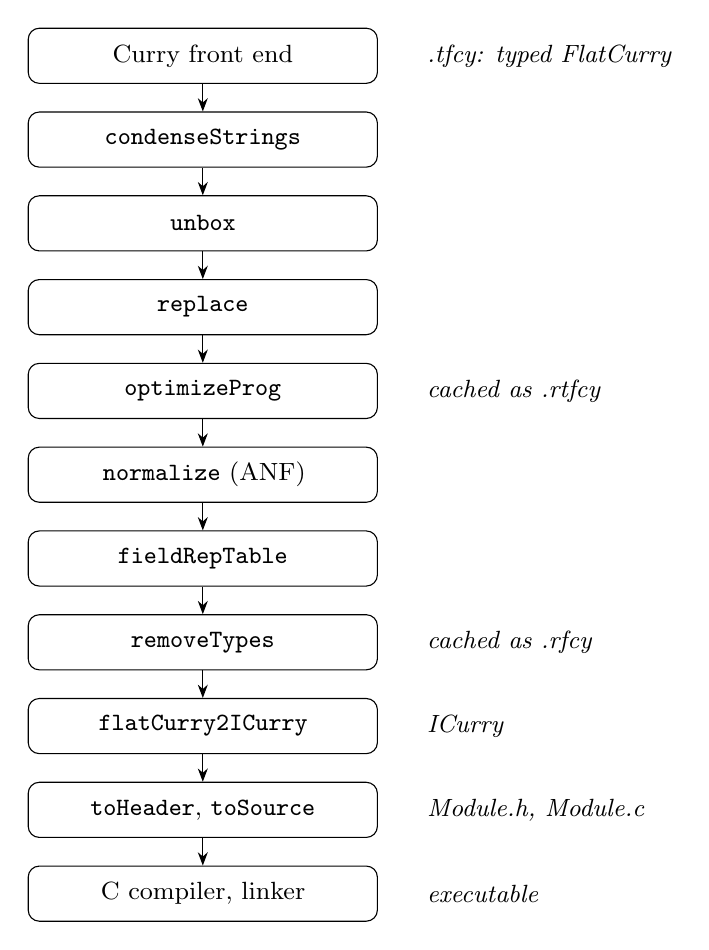
\begin{tikzpicture}[
  pass/.style={draw, rounded corners, text width=4.2cm, align=center,
               minimum height=0.7cm, font=\small},
  data/.style={font=\small\itshape},
  node distance=0.35cm]
  \node[pass] (fe) {Curry front end};
  \node[pass, below=of fe] (str) {\code{condenseStrings}};
  \node[pass, below=of str] (unbox) {\code{unbox}};
  \node[pass, below=of unbox] (rep) {\code{replace}};
  \node[pass, below=of rep] (opt) {\code{optimizeProg}};
  \node[pass, below=of opt] (anf) {\code{normalize} (ANF)};
  \node[pass, below=of anf] (fr) {\code{fieldRepTable}};
  \node[pass, below=of fr] (unt) {\code{removeTypes}};
  \node[pass, below=of unt] (ic) {\code{flatCurry2ICurry}};
  \node[pass, below=of ic] (cg) {\code{toHeader}, \code{toSource}};
  \node[pass, below=of cg] (cc) {C compiler, linker};
  \foreach \a/\b in {fe/str, str/unbox, unbox/rep, rep/opt, opt/anf, anf/fr,
                     fr/unt, unt/ic, ic/cg, cg/cc}
    \draw[-{Stealth}] (\a) -- (\b);
  \node[data, right=0.5cm of fe] {\file{.tfcy}: typed FlatCurry};
  \node[data, right=0.5cm of opt] {cached as \file{.rtfcy}};
  \node[data, right=0.5cm of unt] {cached as \file{.rfcy}};
  \node[data, right=0.5cm of ic] {ICurry};
  \node[data, right=0.5cm of cg] {\file{Module.h}, \file{Module.c}};
  \node[data, right=0.5cm of cc] {executable};
\end{tikzpicture}
\end{center}

\file{Rice/Main.curry} runs these passes on each module, in dependency order:
\code{optimizeModule} runs everything up to the optimizer, and
\code{generateModule} runs the rest.  Then \code{buildExecutable} compiles and
links the C.

Every pass from \code{condenseStrings} through \code{normalize} is a function on
typed FlatCurry (\code{TProg}).  Types matter to us: unboxing and field reps
are both about the type of a value.  We drop them at the last moment, because
ICurry generation wants untyped FlatCurry.

\subsection{The standard library and the front end}
\label{sec:frontend}

Rice compiles programs against its own standard library, \file{lib/}, not the
one of the Curry system it was built with.  \file{lib/} is a copy of KiCS2's,
made by \file{tools/sync-lib.sh}, with the CPP symbol \code{__KICS2__} renamed
to \code{__RICE__}: the runtime implements the externals of the KiCS2
branches.  \file{lib/VERSION} says which KiCS2 it came from.  After a sync,
check whether Prelude's externals still match \file{runtime/ext/Prelude.c} and
\file{replace/}.

\code{Rice.Frontend} runs the front end itself, with \code{-D__RICE__}, and
the load path: the current directory, then \code{CURRYPATH}, then
\file{lib/}.  The front end writes each module's \file{.tfcy} into
\file{.curry/rice-1.0.0/} beside its source, with Rice's own cache files.
The front end executable is \code{RICE_FRONTEND} if that's set, otherwise
\file{bin/curry-frontend}, otherwise the one of the Curry system Rice was
built with, otherwise the first of \code{curry-frontend},
\code{kics2-frontend} and \code{pakcs-frontend} on \code{PATH}.
\file{bin/curry-frontend} is built by \code{make frontend} from the
\file{frontend/} submodule, which pins the version Rice is tested with (3.1.0,
the one KiCS2 3.5 uses).  The front end isn't on Hackage past 2.0.0, so it's
built from source with Stack.  Its \file{.tfcy} format has to be the one the
\code{flatcurry-typed} package reads; to move to a newer front end, check out
its tag in \file{frontend/} and check that.

\subsection{Separate compilation and caching}
\label{sec:caching}

\code{Rice.Build.Deps} finds every module the program imports, and sorts them
so that a module comes after its imports.  \code{Rice.Main.run} then compiles
them in that order, passing along what each later module needs from earlier
ones:
\begin{itemize}
  \item the \emph{function table} of every function so far, so the optimizer can
    inline across modules;
  \item every module's untyped FlatCurry, because ICurry generation looks up
    the types of imported constructors.  Prelude's boxed \code{Int} type only
    exists in our transformed Prelude, not in the Prelude on disk;
  \item the \emph{field reps} of every constructor and function so far.
\end{itemize}

Compiling Prelude takes a long time, so we cache aggressively.  Every module
gets a directory \file{.curry/rice-1.0.0/} next to its source (Prelude's is
\file{lib/.curry/rice-1.0.0/}), holding:
\begin{center}
\begin{tabular}{@{}ll@{}}
\toprule
\file{.rtfcy} & the optimized typed FlatCurry \\
\file{.rfcy} & the untyped FlatCurry after ANF \\
\file{.rimports} & just the module's imports \\
\file{.h}, \file{.c} & the generated C \\
\file{obj-<hash>/} & object files, one directory per compiler and flags \\
\file{rice-main.c} & for the root module only \\
\bottomrule
\end{tabular}
\end{center}

A module is \emph{stale} if its \file{.rtfcy} is missing, or older than its
\file{.tfcy} or than any import's \file{.rtfcy} (\code{needsRecompile}).  A
stale module is compiled from scratch.  Otherwise we read its \file{.rtfcy}
instead of optimizing it, and its \file{.rfcy} instead of running the rest of
the pipeline, and keep its \file{.h} and \file{.c}.  Cache files are only
rewritten when their contents change (\code{writeFileIfChanged}), so an
unchanged result doesn't make the modules importing it stale.

The \file{.rimports} file exists because reading any field of a \code{TProg}
parses the whole \file{.tfcy}, which takes seconds for Prelude.

Object files are cached the same way, in a directory \file{obj-<hash>/} next
to the \file{.c}, where the hash is of the C compiler and its flags (the
runtime's are in \file{runtime/obj-<hash>/}).  So builds with different
\code{--cflags}, \code{--debug} or \code{--gcc} keep separate objects.  A
\file{.o} is rebuilt when its \file{.c}, or any header in \file{runtime/},
is newer, or when the \file{.o.flags} file beside it records a different
compiler and flags (in case of a hash collision).  Each object is compiled to
a temporary file and renamed, so two builds at once can't leave a half-written
one.

The staleness check doesn't know that a module depends on \file{replace/} or on
the compiler itself.  After changing either, delete the caches (\code{tests/run.sh}
does that for Prelude unless you pass \code{--no-clean}) or use
\code{--force-recompile-module=Prelude}.

\subsection{String literals}

The front end represents \code{"hello"} as a list of five \code{Char} literals.
\code{Rice.Transform.StrLit} turns that into one constructor call whose module
is empty and whose name is the string: \code{("", "hello")}.  The code generator
recognizes that name (\code{isStrConst}) and builds the list at run time from a
C string, with \code{toCurryString}.  This keeps long strings from becoming huge
expressions for the optimizer and huge functions in C.

\subsection{Unboxing}
\label{sec:unboxing}

In the runtime, \code{Int}, \code{Char} and \code{Float} are ordinary
one-constructor data types, whose single child is a raw C value.  \code{Int 7}
is a node with symbol \code{Int} and a raw \code{long} 7.  We call the raw types
\texttt{Int\#}, \texttt{Char\#} and \texttt{Float\#}.

\code{Rice.Transform.Unbox} makes these boxes explicit in the program, so later
passes can reason about them and remove them.  For Prelude it replaces the
built-in types with the box types.  In every module it changes two kinds of
expression:
\begin{itemize}
  \item A literal gets a box: \code{4} becomes \code{Int 4}, where the inner
    \code{4} is an \texttt{Int\#}.
  \item A case on a literal becomes a case that takes the box apart, around a
    case on the raw value:
\begin{lstlisting}[language=Curry]
case x of            case x of
  1 -> True            Int x' -> case x' of
  4 -> True    ==>                  1 -> True
                                    4 -> True
                       () -> 1
                       () -> 4
\end{lstlisting}
    The \code{() -> n} branches are dummies.  They aren't well typed, and their
    real pattern is a constructor named \code{("","")}, which no program can
    name.  They list the literals the inner case matches, so the outer case
    knows the possible values when it narrows a free variable.
\end{itemize}

The primitive operations themselves are redefined in
\file{replace/replace_Prim.curry} to take their arguments' boxes apart and call
a raw primitive (next section).

What we do \emph{not} do yet is remove boxes: a worker/wrapper split based on
strictness analysis, which old\_rice did, would let a function like \code{fib}
pass raw integers instead of allocating boxes (\S\ref{sec:planned}).

\subsection{Replacing Prelude functions}
\label{sec:replace}

Some Prelude functions need a different definition for Rice.
\code{Rice.Files.Replace} handles this: for module \code{M}, if
\file{replace/replace_M.curry} exists, each of its functions replaces
the function of the same name in \code{M}, and functions only defined there are
added.  The replacements are renamed into \code{M}, and they go through
\code{condenseStrings} and \code{unbox} first, like \code{M} did.

For Prelude, \file{replace_Prim.curry} is applied first.  It defines
\code{Int}, \code{Char} and \code{Float} as boxes around raw types (which it has
to call \code{Int_SH} and so on, since \texttt{Int\#} isn't a legal Curry name; we
rename them), and defines every arithmetic and comparison function as ``take
the boxes apart, call \code{prim_...}, box the result'':
\begin{lstlisting}[language=Curry]
eqInt x y = fcase x of
              Int x' -> fcase y of
                          Int y' -> prim_eqInt x' y'
\end{lstlisting}
\file{replace_Prelude.curry} holds everything else: generators for free
variables of primitive type, and the unification operators, which are
externals in \file{runtime/ext/Prelude.c}.

A replacement must have the same type as the function it replaces, including
type class constraints, because every call site was compiled against the
original.  A different constraint changes the number of (dictionary)
arguments.

\subsection{The optimizer}

The optimizer is a set of rewrite rules on typed FlatCurry expressions
(\code{Rice.Optimize.Inline}), applied bottom-up until none applies, by the
engine in \file{src/FlatCurry/Transform/Typed/ExecDet.curry}.  A rule is a
total function returning \code{Maybe}: the rewritten expression, the rule's
name (for \code{--trace-optimize}), and how many fresh variables it used.  The
rules are:
\begin{description}[style=nextline]
  \item[\code{reduce}] Inline a saturated call to a small function that isn't a
    loop breaker.
  \item[\code{caseCancel}] A case on a known constructor or literal takes that
    branch.
  \item[\code{inline}] Substitute a \code{let}-bound constructor or literal into
    the body; or a \code{let}-bound case used once, where it would be forced
    anyway.
  \item[\code{deadCode}] Drop unused \code{let} and \code{free} bindings,
    except a \code{let} of type \code{IO}: a \code{do} block's statement can
    become \code{let _ = statement in rest}, and its effect still has to
    happen.
\end{description}

\paragraph{Inlining is safe because nothing is duplicated.}  When we inline a
call, a ground argument (a variable, a literal, a constructor of ground
arguments) is substituted directly, and anything else is bound once with a
\code{let} (\code{subGrounded}).  So a shared expression is still evaluated
once, and a nondeterministic one still makes one choice.  This matters more in
Curry than in Haskell: duplicating \code{x} in \code{let x = 0 ? 1 in x + x}
would change the answers.

\paragraph{Loop breakers.}  Inlining a recursive function never stops.  Rather
than refuse to inline any function in a recursive group, we pick
\emph{loop breakers}: a set of functions that, if never inlined, leaves no
cycle in the call graph.  \code{Rice.Transform.Order} takes each strongly
connected component of the call graph, removes the member with the highest
\code{inlineScore} (a rough cost of inlining it), and repeats on what's left.
This is the same idea as GHC's loop breakers (Peyton Jones and Marlow, ``Secrets
of the Glasgow Haskell Compiler inliner'', JFP 2002).

\paragraph{The function table.}  \code{Rice.Optimize.FunTable} records, for
every function in this module and every module before it, its parameters, body,
size, whether it's external, and whether it's a loop breaker.  A function is
inlinable if it isn't external or a loop breaker, and its body is under 35 AST
nodes.

The optimizer runs before ANF, so there are few \code{let}s for \code{inline}
to work on yet; most of the work is \code{reduce} and \code{caseCancel}.

\subsection{A-normal form}

\code{Rice.Transform.ANF} puts every function body in A-normal form: every
argument of a call or constructor, every case scrutinee and every choice
alternative is a variable or a literal, and everything else is named with a
\code{let}.  (The idea is from Flanagan, Sabry, Duba and Felleisen, ``The
Essence of Compiling with Continuations'', PLDI 1993.)  Two later stages rely
on it: field reps assume every scrutinee is a variable, and an inline primitive
only accepts variables and literals as arguments.

\subsection{Field reps}
\label{sec:fieldreps}

Once we unbox, a node's child can be a raw \texttt{Int\#} instead of a pointer
(\S\ref{sec:nodes}).  The garbage collector must know which, and so must the
code that prints a value.  But C erases that, and ICurry is untyped.  So right
after ANF, while we still have types, \code{Rice.Codegen.FieldReps} computes a
\emph{field rep} (\code{RPtr}, \code{RInt}, \code{RChar} or \code{RFloat}) for
every constructor field, every function parameter, and every variable in every
function body, and carries this table alongside the untyped program.  Only the
three raw types are raw; everything else, type variables included, is a
pointer, because a raw value never instantiates a polymorphic type.

Variable numbers survive into ICurry, so the code generator looks variables up
by number.  ICurry generation also invents functions (next section), and
\code{addLiftedReps} works out their reps from the function they came from.

The table turns into the \code{reps} array of each symbol and each frame
(\S\ref{sec:nodes}, \S\ref{sec:frames}).

Raw values have to stay out of places that only hold pointers, and
\code{lintFieldReps} (\code{--lint-fieldreps}, on with \code{--debug} and in
every test) checks that they do:
\begin{itemize}
  \item every argument matches its parameter's rep;
  \item a partial application has no raw parameters, supplied or missing,
    because \code{apply} only ever fills in pointers;
  \item no choice alternative, free variable, or function result is raw (a
    function node is overwritten by its result, which must be a node);
  \item every case scrutinee is a variable; a constructor case's scrutinee is a
    pointer, and a literal case's is raw;
  \item every use of a variable agrees with its binder, and every literal is
    raw.
\end{itemize}

\subsection{ICurry}

\code{removeTypes} turns typed FlatCurry into untyped FlatCurry, and
\code{flatCurry2ICurryWithProgs} (from the \code{icurry} package) turns that
into ICurry.  An ICurry function body is a \emph{block}: variable declarations,
assignments, and one statement that ends the block.
\begin{lstlisting}[language={}]
block      =  declarations; assignments; statement
assignment =  x = e  |  x[i,...] = e
statement  =  return e
           |  exempt                       -- no branch matches: fail
           |  case x of C1 -> block ...    -- constructor case
           |  case x of l1 -> block ...    -- literal case
e          =  x  |  x[i,...]  |  literal  |  e1 ? e2
           |  f(e,...)  |  C(e,...)          -- calls
           |  partial f(e,...)  |  partial C(e,...)
\end{lstlisting}
\code{x[i,j]} is child \code{j} of child \code{i} of \code{x}.  Variable 0 is
always the node being reduced.  Recursive \code{let}s are declared first and
filled in with \code{x[i] = e} afterwards, which is how cyclic graphs get
built.

On the way, ICurry generation \emph{lifts} every nested case, \code{let} and
\code{free} into a new function, named after the function it came from:
\code{f_CASE0}, \code{f_LET0}, \code{f_FREE0}, \code{f_COMPLEXCASE0}.  A lifted
function's parameters are variables of the original, with the same numbers.
So in the generated code, a function has at most one constructor case, at the
end of its block, and a \code{let} in the middle of a body becomes a call to a
lifted function.

\subsection{Generated code}
\label{sec:generated}

Every module becomes a \file{.h} (\code{Rice.Codegen.C.ToH}) and a \file{.c}
(\code{Rice.Codegen.C.ToC}).  Both are built with the DSL in
\code{Rice.Codegen.C.C}, a thin layer of C syntax over \code{Text.Pretty}.

\paragraph{Names.}  A Curry name becomes \code{Module__name}, with every
character that isn't a letter or digit replaced by \code{_} and a code
(\code{Rice.Codegen.Names}): \code{_US} for \code{_}, \code{_DL} for \code{$},
\code{_EX} for \code{!}, and so on.  So \code{Prelude.$!} is
\code{Prelude___DL_EX}.

\paragraph{The header.}  For every constructor and every function, the header
has
\begin{itemize}
  \item a tag \texttt{\#define} (constructors only), numbered within its type,
    after the five special tags (\S\ref{sec:tags});
  \item a static \code{Symbol}: tag, arity, name, \code{reps} and the
    \code{_hnf} function;
  \item \code{make_X(args..., missing)}, which allocates a node, and
    \code{set_X(root, args..., missing)}, which rewrites \code{root} in place.
    Both are always inlined.  \code{missing} is how many arguments a partial
    application still needs;
  \item for constructors, \code{make_X_free()} and \code{set_X_free(root)},
    which build the constructor with fresh free variables as children, for
    narrowing.
\end{itemize}

\paragraph{Functions.}  Every function \code{f} becomes \code{f_hnf(root, sp)},
which rewrites the node \code{root}, labeled \code{f}, into head normal form
(\S\ref{sec:eval}).  Here is the code for
\begin{lstlisting}[language=Curry]
add Z     y = y
add (S x) y = S (add x y)
\end{lstlisting}
with the debug output left out.  The entry code reads the arguments, pushes the
case's frame, and jumps to the case block:
\begin{lstlisting}
RICE_CC void Ex__add_hnf(union field root, Frame* sp)
{
    GC_SAFE_POINT(root, sp);
    REWRITE_STAMP();
    field v1 = {0};
    field v2 = {0};
    v1 = child_at(root, 0);
    v2 = child_at(root, 1);
    sp = frame_push(sp, &Ex__add_hnf_case0_info);
    SLOT(0) = root;           // the node we're rewriting
    SLOT(1) = v1;             // the scrutinee, as the case began
    SLOT(2) = v1;             // the loop's current scrutinee
    SLOT(3) = v2;             // other variables the branches use
    SLOT(4).i = root.n->nondet;
    MUSTTAIL return Ex__add_hnf_case0(root, sp);
}
\end{lstlisting}
The case block reloads its state from its frame and loops over the scrutinee
until it's a constructor (slot 5 is the scoped-backtracking cutoff,
\S\ref{sec:opts}):
\begin{lstlisting}
static RICE_CC void Ex__add_hnf_case0(union field _root, Frame* sp)
{
    (void)_root;
    field root = SLOT(0);
    field v1 = SLOT(1);
    field _scrutinee = SLOT(2);
    field v2 = SLOT(3);
    bool nondet = SLOT(4).i;
    SCOPED_LOAD_CUTOFF(5);
    while(true)
    {
        nondet |= _scrutinee.n->nondet;
        switch(_scrutinee.n->symbol->tag)
        {
            case FAIL_TAG: ...       // fail root, pop, RETURN()
            case FUNCTION_TAG:       // evaluate it; it returns here
            {
                SCOPED_MARK_CUTOFF();
                SLOT(2) = _scrutinee;
                SLOT(4).i = nondet;
                MUSTTAIL return _scrutinee.n->symbol->hnf(_scrutinee, sp);
            }
            case CHOICE_TAG: ...     // choose() a side, loop
            case FORWARD_TAG: ...    // follow it, loop
            case FREE_TAG: ...       // narrow: Z, with a choice for S
            case Ex__Z_TAG:
            {
                v1 = _scrutinee;
                trail_node(root, nondet);
                REWRITE_STAMP();
                collapse(root, v2);  // root becomes FORWARD y
                sp = frame_pop(sp);
                RETURN();
            }
            case Ex__S_TAG:
            {
                v1 = _scrutinee;
                trail_node(root, nondet);
                REWRITE_STAMP();
                field v3 = {0};
                v3 = child_at(v1, 0);
                set_Ex__add_USLET0(root, v3, v2, 0);
                sp = frame_pop(sp);
                TAIL_CALL(Ex__add_USLET0_hnf);
            }
        }
    }
}
\end{lstlisting}
\code{add_LET0} is the lifted \code{let} that builds \code{add x y} and then
\code{S} around it.  Things to notice:
\begin{itemize}
  \item A frame is the case's whole state, so when the scrutinee's evaluation
    \code{RETURN}s into the case block, the block starts over from its frame.
    Entering from \code{f_hnf} and returning from an evaluation are the same.
  \item Every branch \emph{rewrites} \code{root}: \code{set_X} if it builds a
    node, \code{collapse} if it returns an existing one, \code{fail} if no
    branch matches.  Before it does, \code{trail_node} records the old
    \code{root} on the trail if the rewrite might have to be undone
    (\S\ref{sec:nondet}).
  \item After the rewrite, control leaves with \code{RETURN()} if \code{root}
    is in head normal form, or jumps to \code{root}'s new code if it isn't.
    That's a tail call, so a tail-recursive Curry function doesn't grow
    anything.
  \item The branch reads \code{x} through \code{v1}, which the loop points at
    the constructor it found (\code{writeBack}).  The graph still points at
    the original node: we never point past a FORWARD in the graph
    (\S\ref{sec:forward}).
\end{itemize}
A literal case is an \code{if} chain on the raw value instead of a loop, since a
raw value is already evaluated.

\paragraph{Primitives.}  The \code{prim_...} functions of
\file{replace_Prim.curry} that are pure (arithmetic, comparisons, conversions,
the math library) are in \code{Rice.Codegen.C.PrimOps}.  A call to one compiles
to a C expression on raw values, like \code{(field)(long)(v1.i + v2.i)}, and they get
no symbol or \code{_hnf} function.  Their arguments are always variables or
literals, thanks to ANF.  An inline primitive runs as soon as control reaches
it, which is only right for a pure one; \code{prim_putChar} is an ordinary
external.

\paragraph{Externals.}  A function declared \code{external} has no body in the
generated code.  Its \code{_hnf} is written by hand in
\file{runtime/ext/M.c} for module \code{M}, under its mangled name
(\code{Prelude__prim_USputChar_hnf} in \file{runtime/ext/Prelude.c}); see
\S\ref{sec:externals}.

\subsection{Building the executable}

\code{buildExecutable} writes \file{rice-main.c} for the root module, compiles every
module's \file{.c}, the runtime's \file{.c} files and \file{rice-main.c} with
\code{clang -std=c11 -O2}, and links them into an executable named after the
root module, along with \file{runtime/ext/M.c} for every module \code{M} that
has externals (\code{externalFiles}).  If one of those files is missing, rice
stops and names the module and its externals, before running the C compiler.
\file{rice-main.c} also keeps the command line and Rice's home directory for the
externals.  It initializes the trail, the heap and the machine,
builds a node for \code{main}, and hands it to a driver: \code{run_io}, which
runs an \code{IO} action once, or, with \code{--interactive}, \code{nf_all},
which prints every value \code{main} has (\S\ref{sec:drivers}).

%======================================================================
\section{The runtime system}
\label{sec:runtime}
%======================================================================

We evaluate by \emph{graph rewriting}.  An expression is a graph of nodes.
Evaluating a node rewrites it \emph{in place} with its result, so every other
node that points to it sees the result too.  That's how laziness shares work.
It's also why backtracking is interesting: to try another alternative, we have
to undo those in-place rewrites.

\subsection{Nodes and fields}
\label{sec:nodes}

Every node has the same layout (\file{runtime/node.h}):
\begin{lstlisting}
typedef struct Node
{
    int16_t missing;
    bool nondet;
    unsigned char gc_bits;
    unsigned int epoch;        // only with OPT_EPOCH_TRAIL
    Symbol* symbol;
    union field children[4];
} Node;
\end{lstlisting}
A node is six words, 48 bytes.  The first word holds \code{missing},
\code{nondet}, \code{gc_bits} and \code{epoch}; that's why \code{missing}
is only 16 bits.  Nodes are most of what a program allocates, so a field that
grows the node to seven words costs time everywhere: when \code{missing} was an
\code{int}, turning on \code{OPT_EPOCH_TRAIL} made ReverseBuiltin about 35\%
slower from the extra word alone.

The \code{symbol} points to static information shared by every node of the same
kind: its tag, arity, name, the layout of its children, and the code that
evaluates it.  Changing what a node \emph{is} means changing its symbol and its
children together; that's what ``rewriting in place'' means concretely.

A child isn't always a pointer.  Since we unbox, a node can hold a raw
\code{long}, \code{double} or character directly, so a child is a
\code{union field}:
\begin{lstlisting}
typedef union field
{
    struct Node*  n; // a child node
    union field*  a; // the spill array (children[3] only)
    unsigned long c; // a raw Char
    long          i; // a raw Int
    double        f; // a raw Float
} field;
\end{lstlisting}

Every node has room for four children.  Nearly every node has three or fewer.
When a node has more than three, \code{children[3]} instead points to a
\emph{spill array} holding children 3 and up.  The \code{child_at} macros hide
this: \code{child_at(n, 5)} expands to \code{n.n->children[3].a[2]}.

\paragraph{Field reps.}  The union means we lose track of which children are
pointers.  Evaluation doesn't care, because generated code knows the types, but
the garbage collector does: it must never follow a raw \code{Int} as if it were
a pointer.  So each symbol carries a \code{reps} array, one \code{FieldRep} per
child (\code{R_PTR}, \code{R_INT}, \code{R_CHAR}, \code{R_FLOAT}), computed by
the compiler (\S\ref{sec:fieldreps}).  Almost every child is a pointer, so a
\code{NULL} reps array means ``all pointers'', and only symbols with a raw child
have an array.  We store reps as bytes, because a C11 enum takes four.

\paragraph{The word size.}  The runtime assumes a pointer, a \code{long}, and a
\code{double} all fit in one 8-byte \code{union field}.  That's true on 64-bit
macOS and Linux.  On a 32-bit target it isn't, and a \code{_Static_assert} in
\file{machine.h} stops the build.

\subsection{Tags}
\label{sec:tags}

Every symbol has a tag.  The first five are special (\file{runtime.h}):
\begin{center}
\begin{tabular}{@{}ll@{}}
\toprule
\code{FAIL_TAG} & a failed computation \\
\code{FUNCTION_TAG} & a call that hasn't been evaluated yet \\
\code{CHOICE_TAG} & \code{a ? b} \\
\code{FORWARD_TAG} & an indirection to another node (\S\ref{sec:forward}) \\
\code{FREE_TAG} & an unbound free variable \\
\bottomrule
\end{tabular}
\end{center}
Every tag after these is a constructor of some data type, numbered within its
type, so a case expression can \code{switch} on the tag.  A node is in
\emph{head normal form} when its tag is a constructor (or it has failed): we
know its outermost constructor, but not necessarily anything about its
children.

\subsection{The \code{missing} field}

\code{missing} means three different things:
\begin{itemize}
  \item \code{missing == 0}: an ordinary node, fully applied.
  \item \code{missing > 0}: a partial application, still waiting for
    \code{missing} arguments.  Its last \code{missing} child slots are empty.
  \item \code{missing < 0}: an \emph{apply node}, applying a function to
    \code{-missing} arguments.  Apply nodes have their own layout; see below.
\end{itemize}

\subsection{Argument order}
\label{sec:argorder}

Ordinary nodes store their children \emph{forward}: child 0 is the first
argument.  That's what ICurry's variable accesses assume, so it isn't our
choice.  A partial application's missing arguments are its last slots, in the
order they'll arrive.

Apply nodes are the one exception.  \code{apply(f, v1, v2)} stores \code{f} in
child 0, then its arguments \emph{in reverse}: \code{v2} in child 1 and
\code{v1} in child 2.  An apply node doesn't know \code{f}'s arity, and
reversing puts the newest argument at a fixed index regardless.
\code{apply_hnf} flips them around when it copies them into \code{f}'s forward
layout.  If \code{f} ends up with more arguments than it needs, \code{apply_hnf}
fills it, evaluates it, and applies the result to the rest.

\subsection{Evaluation}
\label{sec:eval}

\paragraph{hnf functions.}  Every function \code{f} in the program compiles to
a C function \code{f_hnf}, which rewrites a node labeled \code{f} into head
normal form.  We always call it through the node's symbol,
\code{root.n->symbol->hnf}, because what a node is changes as we evaluate it.

A case expression is a loop over the scrutinee:
\begin{itemize}
  \item \code{FUNCTION}: evaluate it, and look again.
  \item \code{CHOICE}: \code{choose()} one side (\S\ref{sec:nondet}), and look
    again.
  \item \code{FORWARD}: move to the target, and look again.
  \item \code{FREE}: narrow it (\S\ref{sec:free}), and look again.
  \item \code{FAIL}: \code{root} fails too.
  \item a constructor: take that branch.
\end{itemize}
A branch either rewrites \code{root} with a new node (\code{set_X}), makes
\code{root} forward to an existing node (\code{collapse}), or fails.

\subsection{FORWARD nodes and collapsing rules}
\label{sec:forward}

Some rules don't build anything new.  \code{id x = x} just returns an existing
node, and so do \code{x ? y} once we've picked a side, and a free variable once
it's bound.  We can't make \code{root} \emph{be} that other node, because other
nodes already point at \code{root}.  So \code{root} becomes a FORWARD node, an
indirection to the target.

Two rules about forwards are worth knowing early:
\begin{enumerate}
  \item \textbf{Evaluating a FORWARD does nothing.}  \code{forward_hnf} just
    returns.  Whoever wanted the value chases the forward themselves, in a
    loop.  So after one call to \code{HNF(x)}, \code{x} can still be a
    FORWARD; that's why \code{settle()} exists.
  \item \textbf{Evaluation never shortens a forward chain.}  A forward might be
    undone by backtracking, or carry a \code{nondet} flag that readers need to
    see, so pointing past it in the graph can change the program's meaning.
    The garbage collector is the one place we do remove forwards, under strict
    conditions (\S\ref{sec:elision}).  Path compression (\S\ref{sec:opts}) is
    the other, also under conditions.
\end{enumerate}

\subsection{Normal forms and drivers}
\label{sec:drivers}

A program's result has to be evaluated all the way down, not just to head
normal form.  \code{nf} evaluates every reachable child, and fails the whole
expression if any child fails.  \code{ground_nf} also fails on a free variable.

There are two drivers.  \code{run_io} runs a compiled program's \code{main}
once.  \code{nf_all}, used by \code{rice --interactive}, evaluates a goal,
prints the solution, backtracks, and repeats until there are no more solutions.

%----------------------------------------------------------------------
\subsection{The evaluation machine}
\label{sec:machine}

\paragraph{Why we need our own stack.}  The obvious implementation evaluates a
subexpression with an ordinary C call.  But the C stack has a fixed size set by
the OS, and plenty of Curry programs recurse deeper than that.  \code{foldr}
over a long list isn't a tail call, and tail call optimization can't help with
it.

So we keep our own stack (\file{runtime/machine.h}).  The idea is a continuation
passing transformation.  Code like
\begin{lstlisting}
code...
x = f(args);
more code...
\end{lstlisting}
becomes ``push a frame saying what to do with \code{x}, then jump to
\code{f}''.  When \code{f} finishes, it ``returns'' by jumping to the code in
the frame on top of our stack.  Every transfer of control is a tail call, so
the C stack never grows, and the depth of the evaluation lives on our stack,
which can grow as big as it needs to.

\paragraph{Frames are continuations.}
\label{sec:frames}
A frame is \emph{not} a Curry function's activation record.  It's a saved
continuation: the values the code that pushed it needs once the evaluation it
started is done, plus the code to resume.  In C terms, it's like caller-saved
registers spilled across a call, plus a return address.  In compiler terms,
it's a stack-allocated closure.
\begin{lstlisting}
typedef struct FrameInfo
{
    Code code;                 // what runs when we return to this frame
    unsigned short size;       // how many slots
    const unsigned char* reps; // which slots are pointers (for the GC)
    const char* name;          // for print_machine_stack
} FrameInfo;

typedef struct Frame
{
    const FrameInfo* info;
    union field slots[];
} Frame;
\end{lstlisting}
A \code{FrameInfo} describes one kind of frame, the same way GHC's info tables
do (Peyton Jones, ``Implementing lazy functional languages on stock hardware:
the Spineless Tagless G-machine'', JFP 1992).  Its \code{size} is the state the
continuation needs, which has nothing to do with the function's arity.
\code{$!} takes two arguments but saves three slots (\code{[root, x, nondet]}),
and one function can have several kinds of frame: \code{bindIO} has one while
it evaluates \code{m}, and a different one while \code{f} runs.  In generated
code, each case block has one kind of frame.

\begin{center}
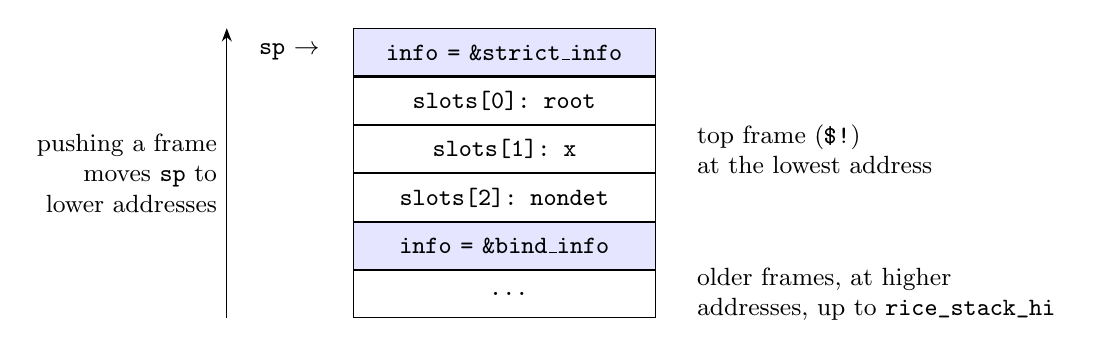
\begin{tikzpicture}[
  word/.style={draw, text width=3.6cm, align=center, minimum height=0.6cm,
               font=\ttfamily\small},
  lab/.style={font=\small}]
  \node[word, fill=blue!10] (h1) {info = \&strict\_info};
  \node[word, below=0pt of h1] (s10) {slots[0]: root};
  \node[word, below=0pt of s10] (s11) {slots[1]: x};
  \node[word, below=0pt of s11] (s12) {slots[2]: nondet};
  \node[word, fill=blue!10, below=0pt of s12] (h2) {info = \&bind\_info};
  \node[word, below=0pt of h2] (s20) {\dots};
  \node[lab, left=0.3cm of h1] {\code{sp} $\rightarrow$};
  \node[lab, right=0.4cm of s11, align=left] {top frame (\texttt{\$!})\\at the lowest address};
  \node[lab, right=0.4cm of s20, align=left] {older frames, at higher\\addresses, up to \code{rice_stack_hi}};
  \draw[-{Stealth}] ($(s20.south west)+(-1.6,0)$) -- ($(h1.north west)+(-1.6,0)$)
     node[midway, left, lab, align=right] {pushing a frame\\moves \code{sp} to\\lower addresses};
\end{tikzpicture}
\end{center}

The stack grows down, so \code{sp} points straight at the top frame's header.
That lets \code{Frame} be a plain struct, and popping a frame only needs its own
\code{size}: \code{frame_pop} returns \code{sp + 1 + size}.  The cost is that
growing the stack can't use \code{realloc}, which keeps data at the
\emph{start} of the block; \code{machine_grow} copies the frames to the top of a
new block instead.  Growing moves the stack, so any old \code{Frame*} is stale
afterwards.

\paragraph{Guaranteed tail calls.}  Machine code transfers control with
\code{MUSTTAIL return f(root, sp);}.  \code{__attribute__((musttail))} makes
the compiler emit a jump instead of a call, at every optimization level, or fail
to compile (see the clang documentation of \code{musttail}).  Without it, the
optimizer is allowed not to, and at \code{-O0} it won't.  \code{musttail}
requires the caller and callee to have the same signature, so every piece of
machine code has the type
\begin{lstlisting}
typedef RICE_CC void (*Code)(union field root, struct Frame* sp);
\end{lstlisting}
even continuations that ignore \code{root}.  That's why \code{RETURN()} passes
\code{NO_ROOT}: a continuation isn't being asked to reduce a new node, so it
reads its own root back out of its frame.

\code{RICE_CC} is \code{__attribute__((preserve_none))} when the compiler
supports it (clang 19 and later).  With the normal C convention, a function
that uses callee-saved registers has to restore them before every tail jump, so
every link in a chain of jumps pays for it.  \code{preserve_none} makes every
register caller-saved, so a jump is just a jump.  It's only worth 0--6\%, and
the runtime is correct without it.

\paragraph{Registers and C code.}  \code{root} and \code{sp} are passed as
arguments to every piece of machine code, so they live in registers.  C code
can't see those.  So there are global copies, \code{rice_root} and
\code{rice_sp}, and two rules:
\begin{itemize}
  \item Before machine code calls C code that might run the machine, it stores
    \code{root} and \code{sp} in the globals.
  \item Afterwards it reloads \code{sp = rice_sp}, because a nested run can grow
    the stack, which moves it.
\end{itemize}
The \code{_hnf} entry points at the bottom of \file{ext/Prelude.c} are this
pattern, written out for each primitive implemented as ordinary C.

\paragraph{Entering and leaving the machine.}  C code runs the machine with
\code{machine_run(code, x)} (or \code{eval_hnf(x)}, which is
\code{machine_run} with \code{x}'s own \code{hnf}).  It pushes a
\emph{sentinel} frame and makes an ordinary C call into \code{code}.
Everything after that is tail jumps.  When the evaluation finishes, the last
\code{RETURN()} lands on the sentinel, whose code stores \code{sp} in
\code{rice_sp} and does a plain \code{return}.  Since there are no C frames in
between, that return comes back out of the call in \code{machine_run}, which
checks that the stack is balanced and pops the sentinel.  Each run pushes its
own sentinel, so C code called from the machine can run the machine again.

\paragraph{Writing a runtime routine for the machine.}  A routine that needs to
evaluate something before it can continue is split in two: the entry point
pushes a frame, and a continuation (by convention \code{foo_k}) does the work.
The continuation starts with \code{EVAL_OR_CONTINUE}: if the value isn't settled
yet, save it in the frame and jump to its code, which returns right back into
the same continuation.  Once it's settled, pop the frame first (after reading
any slots you need, because the next push overwrites them), and finish.
\code{strict_k} for \code{$!} in \file{ext/Prelude.c} is the simplest example.

%----------------------------------------------------------------------
\subsection{Nondeterminism}
\label{sec:nondet}

\paragraph{Choices.}  A choice node is \code{?(left, right, side)}, where
\code{side} is a raw 0 or 1.  \code{choose()} saves a copy of the node on the
trail with \code{side} flipped, and rewrites the node as a FORWARD to the chosen
side.  When we backtrack to it, \code{undo()} puts the saved copy back, and the
next evaluation picks the other side.  Picking the right side pushes an
ordinary entry instead of a choice entry, because there's nothing left to try
after it.

\paragraph{The trail.}  Every in-place rewrite we might need to undo goes on the
\emph{trail} (\file{runtime/trail.h}): a growable array of entries
\code{(lhs, rhs, choice)}, where \code{lhs} is the node we rewrote, and
\code{rhs} is a copy of what it looked like before.

If you know the WAM (A\"it-Kaci, \emph{Warren's Abstract Machine: A Tutorial
Reconstruction}, 1991), here's the surprise: there's no separate choice point
stack.  A choice point is just a trail entry with \code{choice == true}.
\code{undo()} pops entries, copying each \code{rhs} back over its \code{lhs},
until it pops a choice entry, and that's where the search resumes.  The top
level search calls \code{undo(0)}.  Scoped backtracking (\S\ref{sec:opts})
passes a higher cutoff, so it never touches choices older than its own case.

\paragraph{Free variables and narrowing.}
\label{sec:free}
When a case looks at a free variable, we can't take a branch without knowing the
constructor, so we guess.  The generated code for the \code{FREE} case
\begin{enumerate}
  \item pushes an ordinary entry \code{(x -> fresh free variable)}
    (\code{push_frame}), so that once every constructor has been tried,
    \code{x} is free again;
  \item pushes a choice entry for every constructor except the first
    (\code{push_choice});
  \item and rewrites \code{x} as the first constructor, with fresh free
    variables for its arguments (\code{set_X_free}).
\end{enumerate}
A raw child can't be a free variable, so we can't narrow to a constructor with a
raw field yet (\code{narrow_raw_error}).  That includes the boxes, so a free
variable of type \code{Int} can't be narrowed.

\paragraph{Unification.}  \code{x =:= y} (\code{constrEq}) evaluates both
sides to normal form, then walks them together.  A free variable is bound by
turning it into a FORWARD to the other side, and the binding is trailed.  The
result is never \code{False}: if the two sides don't unify, the computation
fails.  Since both sides are evaluated to normal form first, a goal like
\code{x =:= y} where \code{x} has infinitely many values never returns.

\code{x =:<= y} (\code{nonstrictEq}) is the lazy version used for function
patterns.  It only evaluates the left side as far as it needs to.  A free
variable on the left becomes a FORWARD to the (possibly unevaluated) right
side, and a free variable on the right is narrowed to the left side's
constructor.  It runs on the machine, one pair of subterms per frame.

\paragraph{The nondet flag.}  A rewrite only needs to be undone if its result
depends on a choice.  Every node has a \code{nondet} flag.  A choice sets it
when we pick a side, and a case loop ORs in the flag of every node it passes
through, including the forwards, so a function knows whether anything it read
was nondeterministic.  Two consequences are easy to miss: the flag you need is
usually on a node you \emph{passed through}, not the node you ended up on, and
that's another reason the mutator must never skip forwards.

\paragraph{Committing in IO.}  IO never backtracks.  But evaluating an IO
action can still hit a choice (\code{putStrLn "a" ? putStrLn "b"}), and
\code{choose()} pushes an entry.  Once \code{bindIO} moves on, nothing can
reach that choice anymore, but the entry would still be on the trail, and
\code{nf_all} would later backtrack into it and run the program again.  So
\code{bindIO} records the trail's height before it starts, and drops everything
above it (\code{trail_pop_to}, which restores nothing) once it's done.  This
commits to every choice made along the way.

%----------------------------------------------------------------------
\subsection{Making backtracking cheaper}
\label{sec:opts}

Each of these is a compile-time flag in \file{runtime.h}, so we can compare
them.  The design is in \file{src/backtracking-optimizations.md}, and each
combination is proved to give the same answers as the baseline on a model of
the machine; \file{backtracking_proofs.md} says what the implementation has to
do for the proofs to apply.  The generated code is the same for every setting:
the flags only change what the runtime's macros (\code{trail_node},
\code{SCOPED_RETRY}, \code{collapse}, \dots) expand to.

\begin{description}[style=nextline]
  \item[\#1 \code{OPT_NONDET_TRAIL} (on)]
    Only trail a rewrite if it read something nondeterministic.  A
    deterministic rewrite comes out the same no matter which alternative we
    take, so there's nothing to undo.
  \item[\#2 \code{OPT_TAIL_DISPATCH} (on)]
    A tail call jumps straight to the callee's code.  Off, it goes through
    \code{redispatch}, which checks \code{root}'s tag and jumps through its
    symbol, the way a trampoline would.
  \item[\#3 \code{OPT_SCOPED_BACKTRACK} (on)]
    When a case fails, first try to undo choices made since that case started,
    and retry the case, before failing \code{root}.  This keeps a local failure
    from unwinding the whole search.  The cutoff (the trail's height when the
    case started) is recorded lazily, the first time the case might push a
    choice, so a deterministic case pays nothing.
  \item[\#4 \code{OPT_COPY_COLLAPSE} (off)]
    When a collapsing rule's target is a finished value that can't change
    anymore, make \code{root} a copy instead of a FORWARD, which saves every
    reader a hop.
  \item[\#5 \code{OPT_EPOCH_TRAIL} (off)]
    The WAM's trail condition, with time stamps.  Each choice point starts a
    new epoch, and each node remembers the epoch it was created in.  A node
    created after the last choice point becomes unreachable when we backtrack
    past it, so we don't need to trail its rewrites.
  \item[\code{OPT_PATH_COMPRESS} (off)]
    When a case follows a forward, retarget it past the deterministic forwards
    behind it.
  \item[\code{OPT_WRITE_BARRIER} (on exactly when \#1 and \#5 are)]
    Stamp the nodes a deterministic rewrite builds as old as the node they're
    built for.
\end{description}

\#1 and \#5 are each sound alone, but not together: \#1 can leave an old node's
deterministic rewrite untrailed, pointing at a young node whose rewrite \#5
didn't trail.  The write barrier fixes that (\file{opt_conflict.md}), and the
build refuses \#1 and \#5 without it.  \file{current.md} has the latest
measurements.

%----------------------------------------------------------------------
\subsection{Memory and garbage collection}

\paragraph{The heap.}  Nodes and their spill arrays live in a heap made of 4MB
chunks (\file{runtime/heap.c}), allocated with \code{calloc} and kept in a
linked list.  \code{alloc} is an inline bump allocator: it rounds the size up
to 8 bytes and bumps a pointer.  When the current chunk is full, it takes the
slow path, \code{rice_alloc_slow}, which gets a new chunk.

Two things about this are load bearing:
\begin{itemize}
  \item \textbf{Allocation never moves anything.}  C code all over the runtime
    holds raw \code{Node*} pointers that the collector can't see.  One
    contiguous heap would have to grow with \code{realloc}, which can move it.
    New chunks don't.
  \item \textbf{Allocated memory is zeroed.}  Fresh nodes rely on having
    \code{NULL} children, and a spill array's header has to start at 0.
    That's why we use \code{calloc}; it's required for correctness.
\end{itemize}
Everything that isn't a node (the trail, the machine stack, C strings) uses
\code{malloc}.

\paragraph{Safe points.}  Since allocation never collects, when do we collect?
At \emph{safe points}: the start of every \code{_hnf} function
(\code{GC_SAFE_POINT}).  There, every live pointer is somewhere the collector
can find it:
\begin{itemize}
  \item the \code{root} argument;
  \item the slots of every frame on the machine stack, using each frame's
    \code{reps};
  \item the trail;
  \item and \emph{C roots}: local variables in C code that runs the machine
    (\code{eval_hnf}, \code{nf}, \code{settle}, \code{toCStr}), registered with
    \code{GC_ROOT} for as long as they're live.
\end{itemize}
Machine code doesn't need C roots: across an evaluation, its state is in its
frame.  That's one more reason a continuation reads its state from its frame
instead of keeping it in variables.

We collect when the bytes allocated since the last collection pass a threshold.
It starts at 64MB, and after each collection it's set to twice the live data
(but never below 64MB), so collection costs stay proportional to allocation.
The threshold is a soft limit: we can go past it until the next safe point.

\paragraph{The collector.}  The collector (\file{runtime/gc.c}) is a semispace
copying collector over a block-structured heap, like GHC's.  We start a new
chunk list for to-space, copy everything reachable from the roots into it, and
free every chunk in from-space.  To-space grows a chunk at a time, so we never
need to reserve a second heap-sized block.  It traces depth first with an
explicit work stack, rather than Cheney's breadth-first scan, because spill
arrays carry no type information of their own.  (Jones, Hosking and Moss,
\emph{The Garbage Collection Handbook}, covers copying collection.)

Copying a node leaves behind a ``moved'' marker: its symbol becomes
\code{gc_moved_symbol} and its child 0 points to the copy.  A node and its
trail snapshot can share a spill array, so a spill array has a header word in
front of it (at \code{a[-1]}) that records where it was copied to, and both
owners end up sharing the copy.

\paragraph{Removing forwards.}
\label{sec:elision}
A long IO loop makes a long chain of FORWARD nodes.  \code{m >> k} is
\texttt{m >>= \textbackslash\_ -> k}, and the lambda returns \code{k}, an existing node, so the
\code{bindIO} node collapses to \code{FORWARD k}.  Then \code{k} becomes the
next step's \code{bindIO} node, which forwards to the step after that, and so
on.  \code{run_io} holds the first node as a root for the whole run, so every
link stays reachable: one node per iteration, forever.

So when the collector traces a pointer stored \emph{inside a heap node}, it
skips FORWARD nodes that nobody could tell apart from their target, and points
straight at the end of the chain.  This is the same thing GHC's collector does
with indirections.  A forward can be skipped (it's \emph{elidable}) only if it
is
\begin{itemize}
  \item deterministic, because readers collect the \code{nondet} flags of
    forwards they pass through;
  \item and not on the trail, because \code{undo()} might turn it back into
    something else.  The collector marks every trailed node with the
    \code{GC_TRAILED} bit in \code{gc_bits} for the length of a collection.
\end{itemize}
For example, \code{choose()} turns \code{C = ?(l, r)} into \code{FORWARD l} and
trails \code{C}.  If a parent pointing at \code{C} were redirected to \code{l},
then after \code{undo()} restores \code{C} and the search tries \code{r}, the
parent would still see \code{l}.

Roots are never redirected.  Their code may be about to rewrite that exact
node, and redirecting the root would make it rewrite the target instead.  After
walking a chain, we also point every node on it at the end (path compression),
so another pointer into the middle doesn't walk it again.

%----------------------------------------------------------------------
\subsection{External functions}
\label{sec:externals}

The externals of module \code{M} are in \file{runtime/ext/M.c}, named after the
module: \file{ext/Prelude.c}, \file{ext/System.IO.c},
\file{ext/System.Directory.c}, and so on.  \code{Rice.Main} links one whenever
its module is part of the program.  The files for modules outside
\file{lib/}, from packages (\code{System.Directory}, \code{System.Process},
\code{Data.Time}, \code{System.IOExts}, \code{ReadShowTerm}), live here too.

\file{ext/Prelude.c} is the largest.  Its externals are IO (\code{bindIO},
\code{returnIO}, \code{getChar}, \code{prim_putChar}, \code{prim_readFile},
\code{prim_writeFile}, \code{prim_appendFile}), strictness (\code{$!},
\code{$!!}, \texttt{\$\#\#}), \code{&}, \code{cond}, \code{apply},
unification (\code{constrEq}, \code{nonstrictEq}), \code{ensureNotFree},
\code{failed}, \code{prim_error}, and showing and reading literals.  It also has
\code{toCurryString} and \code{toCStr}, which convert strings.

The other files use the helpers in \file{runtime/ext.h}.  \code{EXT(f)} defines
\code{f_hnf} and has it call the body that follows, with \code{root} the call
node.  The body reads the arguments with \code{ext_int}, \code{ext_string},
\code{ext_tag} and so on, which evaluate them, then overwrites \code{root}
with the result (\code{ext_return} and friends).  An IO action is no
different: evaluating it runs it.  Reading an argument runs the machine, which
can collect, so a body keeps \code{root} in a \code{GC_ROOT} until it has read
every argument.

A \code{Handle} (\file{ext/System.IO.c}) is a node with two raw fields, the
\code{FILE*} and whether it can be read and written.  \code{Handle} is an
\code{external data} type, so it has no generated constructor, and
\file{ext/System.IO.c} defines the symbol.

There's no exception handling yet: \code{catch} is a stub, and a failed IO
operation ends the program with the C library's reason
(\code{ext_io_error}).  Stubs that stop with an error (\code{ext_unsupported}):
\code{catch}, \code{System.IOExts}'s commands with pipes, and
\code{ReadShowTerm}, which would need a table of every constructor.  Modules
with externals and no file yet: \code{Data.IORef}, \code{System.IO.Unsafe},
and \code{Control.Search.*}.

Most are written as machine code with a continuation (\code{bind_k},
\code{strict_k}, \code{lu_k}); those are the examples to copy when you write a
new one.

%======================================================================
\section{Testing}
\label{sec:testing}
%======================================================================

\file{tests/run.sh} compiles and runs every program under
\file{tests/programs/}, and compares its output with the \file{.expected} file
next to it, if there is one.  \file{tests/manifest.txt} marks programs that are
skipped, expected to fail, or too slow for every run.  A program can carry
directives in comments: \code{-- rice-mode: interactive},
\code{-- rice-flags: ...}, \code{-- rice-exit: N}, \code{-- rice-maxrss: N} (a
memory limit, for the collector).  Every test is compiled with
\code{--lint-fieldreps}.  \file{tests/README.md} has the details.

The programs come from old\_rice's benchmarks and test suite, KiCS2's
benchmarks, PAKCS's examples, and \file{regressions/}, one program per bug
we've fixed.  When you fix a bug, add the program that found it to
\file{regressions/}, and check that it fails without your fix: the order in
which \code{nf} evaluates things means a program ported from somewhere else
doesn't always exercise the same path.

\file{tests/bench.sh} and \file{tests/optbench.sh} measure speed and count
runtime events across flag settings.  \file{test/runtime_smoke.c} tests the
runtime on its own (\code{make test} in \file{runtime/}).

Two test runs can go at the same time, even with different C flags, as long
as the second passes \code{--no-clean}: a clean start deletes the compiled
Prelude the first run is using.

%======================================================================
\section{Conventions}
%======================================================================

\file{STYLE_GUIDE.md} has the full conventions.  The ones that bite:
\begin{itemize}
  \item \textbf{Use \code{case}, not overlapping equations.}  In Curry, two
    equations whose patterns overlap (a specific one and a catch-all) are
    \emph{both} tried: the function is nondeterministic.  Use separate equations
    only when every pattern is a different constructor of the same type.
    Otherwise write one equation with a \code{case}, which commits to the first
    matching branch.
  \item \textbf{No nondeterminism in Rice itself.}  Rice runs on KiCS2, where
    any nondeterminism costs time even when there's only one answer, and a
    nondeterministic value that reaches IO is an error.  Don't use \code{?} or
    free variables in the compiler.
  \item \textbf{Comments explain the code.}  History goes in the history files,
    and the design in this manual (\S\ref{sec:docs}).
\end{itemize}

%======================================================================
\section{Things that surprise new readers}
%======================================================================

\begin{itemize}
  \item A \code{reps} array that's \code{NULL} means every child is a pointer.
  \item Ordinary nodes store arguments forward; apply nodes store them in
    reverse.
  \item \code{missing} is positive for partial applications and negative for
    apply nodes.
  \item \code{HNF(x)} can leave \code{x} as a FORWARD.  Use \code{settle()} if
    you need a value.
  \item Never point past a FORWARD node in the graph.  Only the collector and
    path compression do that, and only under the conditions above.
  \item A frame is a continuation's saved state, not a function's arguments.
    Read the slots you need before you pop the frame.
  \item After machine code calls C code that might run the machine, reload
    \code{sp = rice_sp}.  The stack may have moved.
  \item A C local holding a node pointer across a call that runs the machine
    has to be a C root (\code{GC_ROOT}), or the collector won't update it.
  \item There's no choice point stack; choice points are entries on the trail.
  \item ICurry lifts every nested \code{let} and case into its own function, so
    the C for one Curry function is spread over several \code{_hnf} functions.
  \item A string literal is a constructor with an empty module name.
  \item The staleness check doesn't track \file{replace/} or the compiler.
    Clear the caches after changing them.
  \item \code{(=:=)} evaluates both sides to normal form first, so a goal with
    infinitely many solutions prints its answers and then never ends.  Output
    is buffered, so it can look like it hangs before printing anything.
\end{itemize}

%======================================================================
\section{Planned work and known gaps}
\label{sec:planned}
%======================================================================

\paragraph{Case shortcutting.}  In \code{case x || y of ...} we don't need a node
for \code{x || y}, only its result.  old\_rice evaluated such scrutinees in one
static node, \code{RET}, instead of allocating.  The hard part is
nondeterminism: if the scrutinee's evaluation reads a choice, something has to
go on the trail, and the trail can't point at a static node that will be reused.
old\_rice's answer was a second entry point \code{f_RET_hnf(backup)} for every
function, which allocates a real node only once a choice shows up.  The
\code{hnf_RET} field of \code{Symbol} and \code{make_restore} in
\file{runtime.h} are placeholders for this.  \file{src/case-shortcutting-plan.md}
has the details, including three designs that don't work.

\paragraph{Removing boxes.}  A strictness analysis, then a worker/wrapper split:
the wrapper unboxes its arguments and calls a worker that takes raw values.
Together with case shortcutting, this takes a function like \code{fib} from
several allocations per call to none.

\paragraph{Deforestation.}  Removing intermediate lists with
\code{foldr}/\code{build} (Gill, Launchbury and Peyton Jones, ``A short cut to
deforestation'', FPCA 1993).  The inliner doesn't inline lambdas, which the
standard rule needs; old\_rice used a combined \code{build_fold} combinator
instead.

\paragraph{Difference lists.}  The usual logic programming difference list,
a list with a free variable as its tail that's filled in by unification, isn't
efficient in Curry.  It relies on binding a free variable being as cheap as
filling in a pointer, and in KiCS2 a free variable is a generator instead.  We
tried them for building the generated C, and dropped them.  Whether Rice, where
binding a variable \emph{is} a pointer update, could make them cheap is still
open.

\paragraph{A limited ANF before the optimizer,} naming calls and scrutinees but
not constructors and literals, would give \code{inline} more to do.

\paragraph{Gaps.}  Narrowing a free variable of a primitive type stops with an
error.  \code{catch}, file IO and the \code{read...Literal} functions are stubs.
The trail can keep old snapshots alive (\file{current.md}).  Constructors with
no children are allocated fresh every time instead of shared.

\end{document}
